%%%%% Magnetisches Feld %%%%%
%% Wien'scher Geschwindugkeitsfilter %%


%Some sample text to be displayed above the first subsection

%\subsection{Prinzip}

%Ein Zyklotron besteht aus Zwei hohlen, halbzylindrischen und Duanden an denen eine Spannung mit unterschiedlichem Vorzeichen anliegt, und darüber bzw. darunter liegende Magneten, die ein homogenes Magnetfeld erzeugen. Zudem gibt es einen Einlass und einen Auslass für Teilchen.

%\begin{wrapfigure}{r}{0.4\textwidth} \label{Zyklo}
%
%	\vspace{-10pt}
%	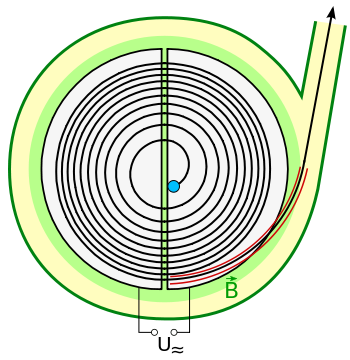
\includegraphics[width=0.35\textwidth]{Zyklotron_Prinzipskizze02.png}
%	\vspace{-13pt}
%	\caption{Prinzipskizze eines Zyklotrons}
%	\vspace{-5pt}	
%	
%\end{wrapfigure}

%\subsubsection{Anwendung}

% Some Formula:

%\begin{equation}
%	x= \frac{y \cdot 13 \pi z}
%			{\cos \alpha}
%\end{equation}

%%%%%%%%%%%%%%%%%%%%%%%
% Eigentlicher Beginn %
%%%%%%%%%%%%%%%%%%%%%%%

Der Wien'sche Geschwindigkeitsfilter ist eine Möglichkeit, einen Elektronenstrahl nach seiner Geschwindigkeit zu filtern, das heißt, nur Elektronen mit einer gewissen Geschwindigkeit passieren zu lassen.

\subsection{Aufbau}

\begin{figure}[h!]
	\centering
	\vspace*{-10pt}
	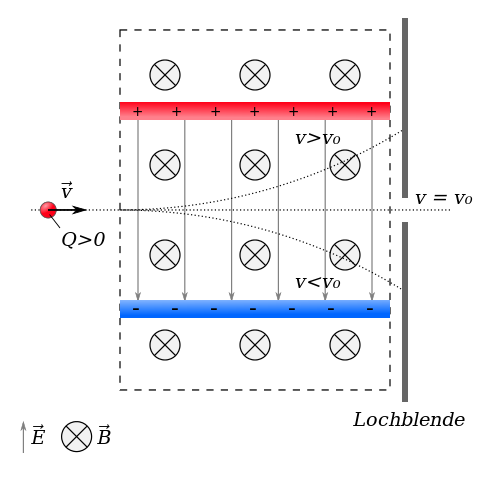
\includegraphics[width=0.6\textwidth]{Wien}
	\caption{Der Geschwindigkeitsfilter nach Wien}
	\label{fig:Wien}
\end{figure}

Grundbaustein bildet eine Ablenkeinheit mit einem Kondensator, wie sie in der Braun'schen Röhre (Siehe: \referenz{sec:BraunscheRoehre}) verwendet wird. Allerdings wird nun ein homogenes Magnetfeld so über den Kondensator gelegt, dass die Feldlinien dieses Feldes senkrecht auf der Elektronenrichtung \emph{und} den Feldlinien des elektrischen Feldes stehen.

Abbildung \ref{fig:Wien} \footnote{„Geschwindigkeitsfilter nach Wien“ von Miessen - Eigenes Werk. Lizenziert unter CC0 über Wikimedia Commons - \url{https://commons.wikimedia.org/wiki/File:Geschwindigkeitsfilter\_nach\_Wien.svg}} zeigt den schematischen Aufbau, jedoch werden positiv geladene Körper ($q>0$) betrachtet und nicht wie hier Elektronen.


\begin{leftbar}
	Anmerkung: Da die magnetischen Feldlinien nicht zeichenbar sind, da sie \glqq in die Papierebene\grqq{} gehen. Dafür wird $\odot$ verwendet, um Anzuzeigen, dass der Pfeil aus der Ebene hinaus verläuft und $\otimes$ um Anzuzeigen, dass der Pfeil in die Ebene hinein verläuft.
	
	Eselsbrücke: Wenn man mit einem Bogen einen Pfeil verschießt, sie man das Kreuz der Federn; im letzten Moment, bevor man von einem getroffen wird, sieht man den Punkt der Pfeilspitze.
\end{leftbar}



\subsection{Funktionsweise}

Das Magnetfeld und der Kondensator werden so gepolt, dass die, gemäß linker Handregel resultierende, Lorentzkraft $F_{Lr}$ der Coulombkraft $F_{el}$ entgegenwirkt. Da die Lorentzkraft abhängig von der Geschwindigkeit des Elektrons ist und die elektrische Kraft nicht, gibt es eine Geschwindigkeit, bei der sich die beiden Kräfte die Waage halten:

\begin{align}
\begin{split}
	F_{Lr} &= F_{el} \\
	q_e \cdot B \cdot v &= q_E \cdot E \\
	v &= \frac{E}{B}
\end{split}
\end{align}

\noindent \emph{Man nehme Notiz von dieser simplen und unglaublich schönen Beziehung!}

Eine Einheitenrechnung folgt:

\begin{align}
\begin{split}
	v &= \frac{E}{B} \\
	\frac{m}{s} &= \frac{N}{C} \cdot \frac{1}{T} \\
	\frac{m}{s} &= \frac{kg \cdot m}{s^2 \cdot As} \cdot \frac{As^2}{kg} \\
	\frac{m}{s} &= \frac{m}{s}
\end{split}
\end{align}


















